\documentclass{article}

  % packages
    % basic stuff for rendering math
    \usepackage[letterpaper, top=1in, bottom=1in, left=1in, right=1in]{geometry}
    \usepackage[utf8]{inputenc}
    \usepackage[english]{babel}
    \usepackage{amsmath} 
    \usepackage{amssymb}

    % extra math symbols and utilities
    \usepackage{mathtools}        % for extra stuff like \coloneqq
    \usepackage{mathrsfs}         % for extra stuff like \mathsrc{}
    \usepackage{centernot}        % for the centernot arrow 
    \usepackage{bm}               % for better boldsymbol/mathbf 
    \usepackage{enumitem}         % better control over enumerate, itemize
    \usepackage{hyperref}         % for hypertext linking
    \usepackage{fancyvrb}          % for better verbatim environments
    \usepackage{newverbs}         % for texttt{}
    \usepackage{xcolor}           % for colored text 
    \usepackage{listings}         % to include code
    \usepackage{lstautogobble}    % helper package for code
    \usepackage{parcolumns}       % for side by side columns for two column code
    

    % page layout
    \usepackage{fancyhdr}         % for headers and footers 
    \usepackage{lastpage}         % to include last page number in footer 
    \usepackage{parskip}          % for no indentation and space between paragraphs    
    \usepackage[T1]{fontenc}      % to include \textbackslash
    \usepackage{footnote}
    \usepackage{etoolbox}

    % for custom environments
    \usepackage{tcolorbox}        % for better colored boxes in custom environments
    \tcbuselibrary{breakable}     % to allow tcolorboxes to break across pages

    % figures
    \usepackage{pgfplots}
    \pgfplotsset{compat=1.18}
    \usepackage{float}            % for [H] figure placement
    \usepackage{tikz}
    \usepackage{tikz-cd}
    \usepackage{circuitikz}
    \usetikzlibrary{arrows}
    \usetikzlibrary{positioning}
    \usetikzlibrary{calc}
    \usepackage{graphicx}
    \usepackage{algorithmic}
    \usepackage{caption} 
    \usepackage{subcaption}
    \captionsetup{font=small}

    % for tabular stuff 
    \usepackage{dcolumn}

    \usepackage[nottoc]{tocbibind}
    \pdfsuppresswarningpagegroup=1
    \hfuzz=5.002pt                % ignore overfull hbox badness warnings below this limit

  % New and replaced operators
    \DeclareMathOperator{\Tr}{Tr}
    \DeclareMathOperator{\Sym}{Sym}
    \DeclareMathOperator{\Span}{span}
    \DeclareMathOperator{\std}{std}
    \DeclareMathOperator{\Cov}{Cov}
    \DeclareMathOperator{\Var}{Var}
    \DeclareMathOperator{\Corr}{Corr}
    \DeclareMathOperator{\pos}{pos}
    \DeclareMathOperator*{\argmin}{\arg\!\min}
    \DeclareMathOperator*{\argmax}{\arg\!\max}
    \newcommand{\ket}[1]{\ensuremath{\left|#1\right\rangle}}
    \newcommand{\bra}[1]{\ensuremath{\left\langle#1\right|}}
    \newcommand{\braket}[2]{\langle #1 | #2 \rangle}
    \newcommand{\qed}{\hfill$\blacksquare$}     % I like QED squares to be black

  % Custom Environments
    \newtcolorbox[auto counter, number within=section]{question}[1][]
    {
      colframe = orange!25,
      colback  = orange!10,
      coltitle = orange!20!black,  
      breakable, 
      title = \textbf{Question \thetcbcounter ~(#1)}
    }

    \newtcolorbox[auto counter, number within=section]{exercise}[1][]
    {
      colframe = teal!25,
      colback  = teal!10,
      coltitle = teal!20!black,  
      breakable, 
      title = \textbf{Exercise \thetcbcounter ~(#1)}
    }
    \newtcolorbox[auto counter, number within=section]{solution}[1][]
    {
      colframe = violet!25,
      colback  = violet!10,
      coltitle = violet!20!black,  
      breakable, 
      title = \textbf{Solution \thetcbcounter}
    }
    \newtcolorbox[auto counter, number within=section]{lemma}[1][]
    {
      colframe = red!25,
      colback  = red!10,
      coltitle = red!20!black,  
      breakable, 
      title = \textbf{Lemma \thetcbcounter ~(#1)}
    }
    \newtcolorbox[auto counter, number within=section]{theorem}[1][]
    {
      colframe = red!25,
      colback  = red!10,
      coltitle = red!20!black,  
      breakable, 
      title = \textbf{Theorem \thetcbcounter ~(#1)}
    } 
    \newtcolorbox[auto counter, number within=section]{proposition}[1][]
    {
      colframe = red!25,
      colback  = red!10,
      coltitle = red!20!black,  
      breakable, 
      title = \textbf{Proposition \thetcbcounter ~(#1)}
    } 
    \newtcolorbox[auto counter, number within=section]{corollary}[1][]
    {
      colframe = red!25,
      colback  = red!10,
      coltitle = red!20!black,  
      breakable, 
      title = \textbf{Corollary \thetcbcounter ~(#1)}
    } 
    \newtcolorbox[auto counter, number within=section]{proof}[1][]
    {
      colframe = orange!25,
      colback  = orange!10,
      coltitle = orange!20!black,  
      breakable, 
      title = \textbf{Proof. }
    } 
    \newtcolorbox[auto counter, number within=section]{definition}[1][]
    {
      colframe = yellow!25,
      colback  = yellow!10,
      coltitle = yellow!20!black,  
      breakable, 
      title = \textbf{Definition \thetcbcounter ~(#1)}
    } 
    \newtcolorbox[auto counter, number within=section]{example}[1][]
    {
      colframe = blue!25,
      colback  = blue!10,
      coltitle = blue!20!black,  
      breakable, 
      title = \textbf{Example \thetcbcounter ~(#1)}
    } 
    \newtcolorbox[auto counter, number within=section]{code}[1][]
    {
      colframe = green!25,
      colback  = green!10,
      coltitle = green!20!black,  
      breakable, 
      title = \textbf{Code \thetcbcounter ~(#1)}
    } 
    \newtcolorbox[auto counter, number within=section]{algo}[1][]
    {
      colframe = green!25,
      colback  = green!10,
      coltitle = green!20!black,  
      breakable, 
      title = \textbf{Algorithm \thetcbcounter ~(#1)}
    } 

    \definecolor{dkgreen}{rgb}{0,0.6,0}
    \definecolor{gray}{rgb}{0.5,0.5,0.5}
    \definecolor{mauve}{rgb}{0.58,0,0.82}
    \definecolor{darkblue}{rgb}{0,0,139}
    \definecolor{lightgray}{gray}{0.93}
    \renewcommand{\algorithmiccomment}[1]{\hfill$\triangleright$\textcolor{blue}{#1}}

    % default options for listings (for code)
    \lstset{
      autogobble,
      frame=ltbr,
      language=Python,
      aboveskip=3mm,
      belowskip=3mm,
      showstringspaces=false,
      columns=fullflexible,
      keepspaces=true,
      basicstyle={\small\ttfamily},
      numbers=left,
      firstnumber=1,                        % start line number at 1
      numberstyle=\tiny\color{gray},
      keywordstyle=\color{blue},
      commentstyle=\color{dkgreen},
      stringstyle=\color{mauve},
      backgroundcolor=\color{lightgray}, 
      breaklines=true,                      % break lines
      breakatwhitespace=true,
      tabsize=3, 
      xleftmargin=2em, 
      framexleftmargin=1.5em, 
      stepnumber=1
    }

  % Page style
    \pagestyle{fancy}
    \fancyhead[L]{AP Calc AB}
    \fancyhead[C]{Muchang Bahng}
    \fancyhead[R]{Spring 2025} 
    \fancyfoot[C]{\thepage / \pageref{LastPage}}
    \renewcommand{\footrulewidth}{0.4pt}          % the footer line should be 0.4pt wide
    \renewcommand{\thispagestyle}[1]{}  % needed to include headers in title page

\begin{document}

\title{AP Calculus AB}
\author{Muchang Bahng}
\date{Spring 2025}

\maketitle

\section{Review}

  So far, we've learned that a \textbf{derivative} is the limit defined 
  \begin{equation}
    \frac{df}{dx} = f^\prime (x) = \lim_{h \rightarrow 0} \frac{f(x + h) - f(x)}{h}
  \end{equation}

  An \textbf{indefinite integral} is simply the opposite of a derivative in that if the derivative of $f(x)$ is another function $f^\prime (x) = g(x)$, then we can take the indefinite integral on $g(x)$ to get back the original function $f(x)$.\footnote{Don't forget the $+c$!}
  \begin{equation}
    \int f^\prime (x) \,dx = \int g(x) \,dx = f(x) + c 
  \end{equation}
  On the other hand, a \textbf{definite integral}, which has two numbers called the \textbf{limits of integration} $a$ and $b$, represent the signed (positive or negative) area under the curve $f(x)$. 
  \begin{equation}
    \int_a^b f(x) \,dx
  \end{equation}
  At first glance, it seems like the definite integral and indefinite integral have nothing to do with each other. One is the anti-derivative and the other is used to calculate areas of curvy shapes. But they are connected by the \textbf{fundamental theorem of calculus} (which is really two theorems), which I will explain now. First, let's play a game. Say that I give you a function $f(t)$, and I tell you also some starting point $t=a$. I want you to give me a function, let's call it $F(x)$, which computes the area under the curve of $f(t)$ from $t=a$ to $t=x$. That is, it is a function that takes in an input $x$, and it spits out a number that is equal to the area of $f(t)$ from $t=a$ to $t=b$. We can use definite integrals for this and see that 
  \begin{equation}
    F(x) = \int_a^x f(t)\,dt
  \end{equation}
  If you're having a hard time understanding this, look at the figure below. This is the \textit{first fundamental theorem of calculus}. Note that while the lower limit of integration $a$ is a constant, the upper limit is a variable! 

  \begin{figure}[H]
    \centering 
    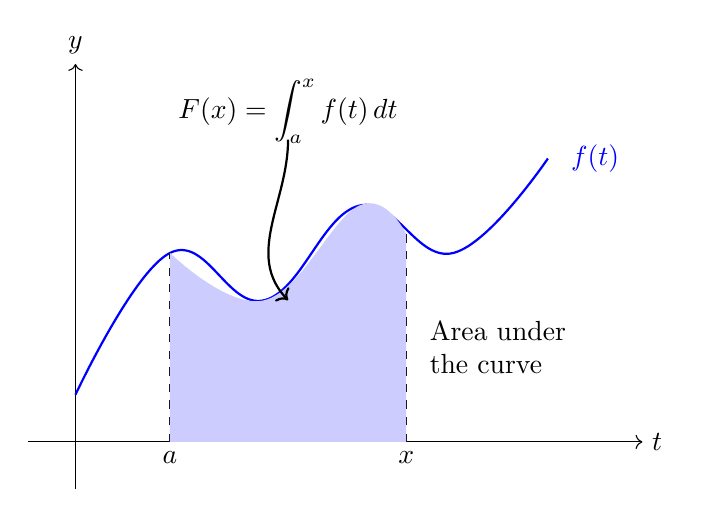
\begin{tikzpicture}[scale=1.2]
      % Define the function using a smooth curve
      \draw[->] (-0.5,0) -- (6,0) node[right] {$t$};
      \draw[->] (0,-0.5) -- (0,4) node[above] {$y$};
      
      % Draw the function curve
      \draw[thick, blue] plot[smooth, tension=0.7] 
          coordinates {(0,0.5) (1,2) (2,1.5) (3,2.5) (4,2) (5,3)};
      
      % Label the curve
      \node[blue] at (5.5,3) {$f(t)$};
      
      % Draw the bounds
      \draw[dashed] (1,0) -- (1,2);
      \draw[dashed] (3.5,0) -- (3.5,2.2);
      
      % Label the bounds
      \node[below] at (1,0) {$a$};
      \node[below] at (3.5,0) {$x$};
      
      % Shade the area
      \fill[blue!20] plot[smooth, tension=0.7] 
          coordinates {(1,2) (2,1.5) (3,2.5) (3.5,2.2)} 
          -- (3.5,0) -- (1,0) -- cycle;
      
      % Add the integral label
      \node at (2.25,3.5) {$F(x) = \displaystyle\int_a^x f(t)\,dt$};
      
      % Add arrow pointing to shaded area
      \draw[->, thick] (2.25,3.2) to[out=-90,in=135] (2.25,1.5);
      
      % Add descriptive text
      \node[text width=3cm] at (5,1) {Area under\\the curve};
    \end{tikzpicture}
    \caption{The integral shows the area under the curve. Apologize for the shading of the area not matching exactly as the function.} 
    \label{fig:first}
  \end{figure}

  This is our input to the function $F(x)$, not $t$! Now let's make the game harder. Say that I give you a function $f(t)$, along with a starting point $t=a$ and an end point $t=b$. I want you to give me a function, let's call it $G(a, b)$, which computes the area under the curve of $f(t)$ from $t=a$ to $t=b$. In other words, it is a function that takes in \textit{two} inputs $a$ and $b$, and it spits out a number that is equal to the area of $f(t)$ from $t=a$ to $t=b$. This may sound a lot harder than the previous problem, but there is a simple solution! Imagine that there is a number $c$ that is less than $a$ and $b$, so $c < a < b$. Then, we can use our previous function $F(a)$, which calculates the area of $f(t)$ from $t=c$ to $t=a$, and the same function again $F(b)$, which calculates the area of $f(t)$ from $t=c$ to $t=b$. 
  \begin{align}
    F(a) & = \int_c^a f(t)\,dt \\
    F(b) & = \int_c^b f(t)\,dt 
  \end{align} 
  Then we can visualize that the area of $f(t)$ from $t=a$ to $t=b$ \textit{must} be $F(b) - F(a)$! Look at the figure below if you are having a hard time visualizing it. Therefore, this gives us our \textit{second fundamental theorem of calculus}. In other words, it states that the definite integral of $f(x)$ can be calculated by taking the indefinite integral of $f(x)$, which we call $F(x)$, and then computing $F(b) - F(a)$. 
  \begin{equation}
    \int_a^b f(x) \,dx = F(x) \big|_a^b = F(b) - F(a)
  \end{equation} 
  Look at the figure below 

  \begin{figure}[H]
    \centering 
    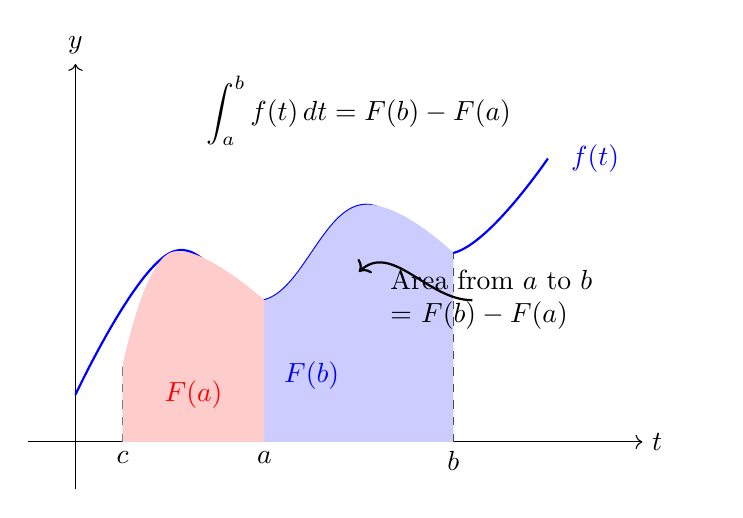
\begin{tikzpicture}[scale=1.2]
      % Define axes
      \draw[->] (-0.5,0) -- (6,0) node[right] {$t$};
      \draw[->] (0,-0.5) -- (0,4) node[above] {$y$};
      
      % Draw the function curve
      \draw[thick, blue] plot[smooth, tension=0.7] 
          coordinates {(0,0.5) (1,2) (2,1.5) (3,2.5) (4,2) (5,3)};
      
      % Label the curve
      \node[blue] at (5.5,3) {$f(t)$};
      
      % Draw vertical lines for c, a, and b
      \draw[dashed] (0.5,0) node[below] {$c$} -- (0.5,0.8);
      \draw[dashed] (2,0) node[below] {$a$} -- (2,1.5);
      \draw[dashed] (4,0) node[below] {$b$} -- (4,2);
      
      % First shade the area from c to b (blue)
      \fill[blue!20] plot[smooth, tension=0.7] 
          coordinates {(0.5,0.8) (1,2) (2,1.5) (3,2.5) (4,2)} 
          -- (4,0) -- (0.5,0) -- cycle;
          
      % Then shade the area from c to a (red) on top
      \fill[red!20] plot[smooth, tension=0.7] 
          coordinates {(0.5,0.8) (1,2) (2,1.5)} 
          -- (2,0) -- (0.5,0) -- cycle;
      
      % Add labels for the areas
      \node[red] at (1.25,0.5) {$F(a)$};
      \node[blue] at (2.5,0.7) {$F(b)$};
      
      % Add the difference area label
      \node[text width=4cm] at (5,1.5) {Area from $a$ to $b$\\= $F(b) - F(a)$};
      
      % Add arrow pointing to the difference area
      \draw[->, thick] (4.2,1.5) to[out=180,in=45] (3,1.8);
      
      % Add the equation at the top
      \node at (3,3.5) {$\displaystyle\int_a^b f(t)\,dt = F(b) - F(a)$};
    \end{tikzpicture}
    \caption{} 
    \label{fig:}
  \end{figure}

\section{Integration By Substitution}

  Solving areas under curves using definite integrals, believe it or not, is very useful. Therefore, we just want to find a bunch of rules for computing these areas, and \textbf{integration by substitution}, also called \textbf{u-substitution}, is one such rule. By the fundamental theorem of calculus, we must compute indefinite integrals before computing definite integrals, so let's focus on indefinite integrals. 

  Remember the chain rule. 
  \begin{equation}
    \frac{d}{dx} f(g(x)) = f^\prime (g(x)) \, g^\prime (x)
  \end{equation}
  Since the indefinite integral is the antiderivative, if we find a function of form $h(x) = f^\prime (g(x)) \, g^\prime (x)$, we can see that 
  \begin{equation}
    \int h(x) \,dx = \int f^\prime (g(x)) \, g^\prime (x) \,dx = f(x) + c
  \end{equation} 
  since we already know the derivative of $f(g(x))$ is $h(x) = f^\prime (g(x)) \, g^\prime(x)$. 

  \begin{definition}[U-Substitution of Indefinite Integrals]
    If we have an integral of the form where $f(x)$ and $u(x)$ are functions. 
    \begin{equation}
      \int h(x) \,dx = \int f(u(x)) \, u^\prime(x) \,dx
    \end{equation} 
    To perform u-substitution, do the following. 
    \begin{enumerate}
      \item \textit{Decompose}. The hardest step is \textit{knowing} that $h(x)$ can be written in the form $f(u(x)) \, u^\prime (x)$. Therefore, you must identify the functions $f(x)$ and $u(x)$ explicitly. We will show how to do this later. 

      \item \textit{Differentiate}. Take $u(x)$ and compute the derivative $u^\prime = g^\prime (x)$. We see that 
      \begin{equation}
        \frac{du}{dx} = u^\prime \implies du = u^\prime (x) \,dx
      \end{equation} 
      Often, we write $u^\prime (x)$ as just $u^\prime$, so the last line is $du = u^\prime \,dx$. 

      \item \textit{Substitute}. Substitute the $u(x)$ with the variable $u$ and $u^\prime (x) \,dx$ with $du$. This gives us 
      \begin{equation}
        \int f(\underbrace{u(x)}_{u}) \, \underbrace{u^\prime(x) \,dx}_{du} = \int f(u) \,du
      \end{equation} 

      \item \textit{Integrate}. Calculate the simplified integral. 
      \begin{equation}
        F(u) = \int f(u) \,du
      \end{equation}

      \item \textit{Substitute Back}. Note that $F(u)$ is a function of $u$, not the original variable $x$. So we substitute $u(x)$ to get a function of $x$. 
      \begin{equation}
        F(u(x))
      \end{equation}
    \end{enumerate}
  \end{definition}

  Now let's talk about for definite integrals. It is very similar to that of the indefinite integral the substitute step has one more part. 

  \begin{definition}[U-Substitution of Definite Integrals]
    If we have an integral of the form where $f(x)$ and $u(x)$ are functions. 
    \begin{equation}
      \int_a^b h(x) \,dx = \int_a^b f(u(x)) \, u^\prime(x) \,dx
    \end{equation} 
    To perform u-substitution, do the following. 
    \begin{enumerate}
      \item \textit{Decompose}. The hardest step is \textit{knowing} that $h(x)$ can be written in the form $f(u(x)) \, u^\prime (x)$. Therefore, you must identify the functions $f(x)$ and $u(x)$ explicitly. We will show how to do this later. 

      \item \textit{Differentiate}. Take $u(x)$ and compute the derivative $u^\prime = g^\prime (x)$. We see that 
      \begin{equation}
        \frac{du}{dx} = u^\prime \implies du = u^\prime (x) \,dx
      \end{equation} 
      Often, we write $u^\prime (x)$ as just $u^\prime$, so the last line is $du = u^\prime \,dx$. 

      \item \textit{Substitute}. Substitute the $u(x)$ with the variable $u$ and $u^\prime (x) \,dx$ with $du$. \textit{In addition}, substitute $a$ with $u(a)$ and $b$ with $u(b)$. This gives us 
      \begin{equation}
        \int_a^b f(\underbrace{u(x)}_{u}) \, \underbrace{u^\prime(x) \,dx}_{du} = \int_{u(a)}^{u(b)} f(u) \,du
      \end{equation} 
      Note that the limits of integration have changed!

      \item \textit{Integrate}. Calculate the simplified integral. Note that this is just a number, so we don't have to substitute back to the variable $x$. 
      \begin{equation}
        \int_{u(a)}^{u(b)} f(u) \,du
      \end{equation}
    \end{enumerate}
  \end{definition}

  This is it! Finally, note that to compute a definite integral using u-substitution, we can actually do it in 2 ways. Both give you the same answer.  
  \begin{enumerate}
    \item Use the u-substitution of definite integrals rule directly. This is the recommended way. 
    \item Compute the indefinite integral $F(x)$ using the u-substitution of indefinite integrals rule, and then just calculate $F(b) - F(a)$. 
  \end{enumerate}

  Now let's go over some examples. 

  \begin{exercise}
    Calculate 
    \begin{equation}
      \int 5 e^{5x} \,dx
    \end{equation}
  \end{exercise}
  \begin{solution}
    To solve $\int 5e^{5x} \,dx$, we'll use u-substitution. Looking at this integral, we notice that there's both a factor of 5 and $e^{5x}$, which suggests we should focus on the $5x$ term.
    
    \textit{Decompose:}
    \begin{itemize}
      \item Our integral $h(x) = 5e^{5x}$ has a form that resembles the chain rule
      \item We can see $5x$ appears in the exponent, so let's set $u(x) = 5x$
      \item Then $f(u) = e^u$ will be our outer function
      \item This decomposition works because $5e^{5x} = e^{5x} \cdot 5 = f(u(x)) \cdot u'(x)$
    \end{itemize}

    \textit{Differentiate:}
    \begin{align*}
      u &= 5x && \text{(our substitution)} \\
      \frac{du}{dx} &= 5 && \text{(derivative of $u$ with respect to $x$)} \\
      du &= 5\,dx && \text{(rearranged to solve for $dx$)}
    \end{align*}

    \textit{Substitute:}
    Now we can rewrite our integral in terms of $u$:
    \begin{align*}
      \int 5e^{5x} \,dx &= \int e^u \,du && \text{(replaced $5x$ with $u$ and $5\,dx$ with $du$)}
    \end{align*}

    \textit{Integrate:}
    \begin{align*}
      \int e^u \,du &= e^u + C && \text{(basic integral of $e^u$)} \\
      &= e^{5x} + C && \text{(substituted back $u = 5x$)}
    \end{align*}

    Therefore, $\int 5e^{5x} \,dx = e^{5x} + C$.
  \end{solution}

  \begin{exercise}
    Calculate 
    \begin{equation}
      \int (x^2 + 1) \cdot x \,dx 
    \end{equation}
  \end{exercise}
  \begin{solution}
    To solve $\int (x^2 + 1) \cdot x \,dx$, we'll use u-substitution. Notice that one factor ($x$) is the derivative of the other factor $(x^2 + 1)$ up to a constant, which suggests a substitution.
    
    \textit{Decompose:}
    \begin{itemize}
      \item Our integral $h(x) = (x^2 + 1) \cdot x$ has a form where one part appears to be the derivative of another
      \item Let's set $u(x) = x^2 + 1$ since we see this expression as a factor
      \item Then $f(u) = u$ will be our function of $u$
      \item Notice that the remaining $x$ factor will relate to $du$ (shown in next step)
    \end{itemize}

    \textit{Differentiate:}
    \begin{align*}
      u &= x^2 + 1 && \text{(our substitution)} \\
      \frac{du}{dx} &= 2x && \text{(derivative of $u$ with respect to $x$)} \\
      du &= 2x\,dx && \text{(therefore)} \\
      x\,dx &= \frac{1}{2}du && \text{(solved for $x\,dx$)}
    \end{align*}

    \textit{Substitute:}
    Now we can rewrite our integral with everything in terms of $u$:
    \begin{align*}
      \int (x^2 + 1) \cdot x \,dx &= \int u \cdot \frac{1}{2}du && \text{(replaced $x^2 + 1$ with $u$ and $x\,dx$ with $\frac{1}{2}du$)} \\
      &= \frac{1}{2}\int u \,du && \text{(factored out constant)}
    \end{align*}

    \textit{Integrate:}
    \begin{align*}
      \frac{1}{2}\int u \,du &= \frac{1}{2} \cdot \frac{u^2}{2} + C && \text{(basic power rule)} \\
      &= \frac{1}{4}u^2 + C \\
      &= \frac{1}{4}(x^2 + 1)^2 + C && \text{(substituted back $u = x^2 + 1$)}
    \end{align*}

    Therefore, $\int (x^2 + 1) \cdot x \,dx = \frac{1}{4}(x^2 + 1)^2 + C$.
  \end{solution}

  \begin{exercise}
    Calculate 
    \begin{equation}
      \int_0^1 (x^2 + 1)^3 \cdot x \,dx 
    \end{equation}
  \end{exercise}
  \begin{solution}
    To solve $\int_0^1 (x^2 + 1)^3 \cdot x \,dx$, we'll use u-substitution. This integral is similar to the previous one, but with a cube power and definite bounds.
    
    \textit{Decompose:}
    \begin{itemize}
      \item Our integral $h(x) = (x^2 + 1)^3 \cdot x$ has a similar structure to the previous problem
      \item Let's set $u(x) = x^2 + 1$ since we see this expression being cubed
      \item Then $f(u) = u^3$ will be our function of $u$
      \item Again, the remaining $x$ factor will relate to $du$
    \end{itemize}

    \textit{Differentiate:}
    \begin{align*}
      u &= x^2 + 1 && \text{(our substitution)} \\
      \frac{du}{dx} &= 2x && \text{(derivative of $u$ with respect to $x$)} \\
      du &= 2x\,dx && \text{(therefore)} \\
      x\,dx &= \frac{1}{2}du && \text{(solved for $x\,dx$)}
    \end{align*}

    \textit{Substitute:}
    For definite integrals, we also need to change the bounds:
    \begin{itemize}
      \item When $x = 0$: $u = 0^2 + 1 = 1$
      \item When $x = 1$: $u = 1^2 + 1 = 2$
    \end{itemize}
    
    Now we can rewrite our integral:
    \begin{align*}
      \int_0^1 (x^2 + 1)^3 \cdot x \,dx &= \int_1^2 u^3 \cdot \frac{1}{2}du && \text{(with new bounds)} \\
      &= \frac{1}{2}\int_1^2 u^3 \,du && \text{(factored out constant)}
    \end{align*}

    \textit{Integrate:}
    \begin{align*}
      \frac{1}{2}\int_1^2 u^3 \,du &= \frac{1}{2}\left[\frac{u^4}{4}\right]_1^2 && \text{(power rule)} \\
      &= \frac{1}{2}\left(\frac{16}{4} - \frac{1}{4}\right) && \text{(evaluated at bounds)} \\
      &= \frac{1}{2} \cdot \frac{15}{4} \\
      &= \frac{15}{8}
    \end{align*}

    Therefore, $\int_0^1 (x^2 + 1)^3 \cdot x \,dx = \frac{15}{8}$.
  \end{solution}

  \begin{exercise}
    Calculate 
    \begin{equation}
      \int \sqrt{2x - 1} \,dx 
    \end{equation}
  \end{exercise}
  \begin{solution}
    To solve $\int \sqrt{2x - 1} \,dx$, we'll use u-substitution. The square root suggests making what's inside it our $u$.
    
    \textit{Decompose:}
    \begin{itemize}
      \item Our integral $h(x) = \sqrt{2x - 1}$ contains a square root
      \item Let's set $u(x) = 2x - 1$ to simplify what's inside the square root
      \item Then $f(u) = \sqrt{u} = u^{\frac{1}{2}}$ will be our function of $u$
      \item The factor of 2 in $2x - 1$ will relate to $du$
    \end{itemize}

    \textit{Differentiate:}
    \begin{align*}
      u &= 2x - 1 && \text{(our substitution)} \\
      \frac{du}{dx} &= 2 && \text{(derivative of $u$ with respect to $x$)} \\
      du &= 2\,dx && \text{(therefore)} \\
      dx &= \frac{1}{2}du && \text{(solved for $dx$)}
    \end{align*}

    \textit{Substitute:}
    \begin{align*}
      \int \sqrt{2x - 1} \,dx &= \int \sqrt{u} \cdot \frac{1}{2}du && \text{(replaced $2x - 1$ with $u$ and $dx$ with $\frac{1}{2}du$)} \\
      &= \frac{1}{2}\int u^{\frac{1}{2}} \,du && \text{(rewrote square root as power)}
    \end{align*}

    \textit{Integrate:}
    \begin{align*}
      \frac{1}{2}\int u^{\frac{1}{2}} \,du &= \frac{1}{2} \cdot \frac{2}{3}u^{\frac{3}{2}} + C && \text{(power rule with $\frac{1}{2} + 1 = \frac{3}{2}$)} \\
      &= \frac{1}{3}u^{\frac{3}{2}} + C \\
      &= \frac{1}{3}(2x - 1)^{\frac{3}{2}} + C && \text{(substituted back $u = 2x - 1$)}
    \end{align*}

    Therefore, $\int \sqrt{2x - 1} \,dx = \frac{1}{3}(2x - 1)^{\frac{3}{2}} + C$.
  \end{solution}

  \begin{exercise}
    Calculate 
    \begin{equation}
      \int_{\pi/3}^{\pi/2} \sin^2 (3x) \, \cos(3x) \,dx
    \end{equation}
  \end{exercise}
  \begin{solution}
    To solve $\int_{\pi/3}^{\pi/2} \sin^2(3x) \cos(3x) \,dx$, we'll use u-substitution. Notice this looks like a power of sine times its derivative (up to a constant).
    
    \textit{Decompose:}
    \begin{itemize}
      \item Our integral $h(x) = \sin^2(3x) \cos(3x)$ contains a power of sine times cosine
      \item Let's set $u(x) = \sin(3x)$ since we see its power
      \item Then $f(u) = u^2$ will be our function of $u$
      \item The $\cos(3x)$ term will relate to $du$ (which makes sense as it's the derivative of sine)
    \end{itemize}

    \textit{Differentiate:}
    \begin{align*}
      u &= \sin(3x) && \text{(our substitution)} \\
      \frac{du}{dx} &= 3\cos(3x) && \text{(derivative using chain rule)} \\
      du &= 3\cos(3x)\,dx && \text{(therefore)} \\
      \cos(3x)\,dx &= \frac{1}{3}du && \text{(solved for $\cos(3x)\,dx$)}
    \end{align*}

    \textit{Substitute:}
    For the definite integral, we need to change the bounds:
    \begin{itemize}
      \item When $x = \frac{\pi}{3}$: $u = \sin(\pi) = 0$
      \item When $x = \frac{\pi}{2}$: $u = \sin(\frac{3\pi}{2}) = -1$
    \end{itemize}
    
    Now we can rewrite our integral:
    \begin{align*}
      \int_{\pi/3}^{\pi/2} \sin^2(3x) \cos(3x) \,dx &= \int_0^{-1} u^2 \cdot \frac{1}{3}du && \text{(with new bounds)} \\
      &= \frac{1}{3}\int_0^{-1} u^2 \,du && \text{(factored out constant)}
    \end{align*}

    \textit{Integrate:}
    \begin{align*}
      \frac{1}{3}\int_0^{-1} u^2 \,du &= \frac{1}{3}\left[\frac{u^3}{3}\right]_0^{-1} && \text{(power rule)} \\
      &= \frac{1}{3}\left(-\frac{1}{3} - 0\right) && \text{(evaluated at bounds)} \\
      &= -\frac{1}{9}
    \end{align*}

    Therefore, $\int_{\pi/3}^{\pi/2} \sin^2(3x) \cos(3x) \,dx = -\frac{1}{9}$.
  \end{solution}

  \begin{exercise}
    Calculate 
    \begin{equation}
      \int_1^5 \frac{x}{\sqrt{2x - 1}} \,dx
    \end{equation}
  \end{exercise}
  \begin{solution}
    To solve $\int_1^5 \frac{x}{\sqrt{2x - 1}} \,dx$, we'll use u-substitution. The expression under the square root in the denominator suggests our substitution.
    
    \textit{Decompose:}
    \begin{itemize}
      \item Our integral $h(x) = \frac{x}{\sqrt{2x - 1}}$ has a square root in the denominator
      \item The expression $2x - 1$ appears in the square root, suggesting we let $u(x) = 2x - 1$
      \item We need to express both $x$ and $dx$ in terms of $u$
      \item From $u = 2x - 1$, we can solve for $x$: $x = \frac{u+1}{2}$
      \item Therefore, our integrand will become $\frac{(u+1)/2}{\sqrt{u}}$ after substitution
    \end{itemize}

    \textit{Differentiate:}
    \begin{align*}
      u &= 2x - 1 && \text{(our substitution)} \\
      \frac{du}{dx} &= 2 && \text{(derivative of $u$ with respect to $x$)} \\
      du &= 2\,dx && \text{(therefore)} \\
      dx &= \frac{1}{2}du && \text{(solved for $dx$)}
    \end{align*}

    \textit{Substitute:}
    For the definite integral, we need to change the bounds:
    \begin{itemize}
      \item When $x = 1$: $u = 2(1) - 1 = 1$
      \item When $x = 5$: $u = 2(5) - 1 = 9$
    \end{itemize}
    
    Now we can rewrite our integral:
    \begin{align*}
      \int_1^5 \frac{x}{\sqrt{2x - 1}} \,dx &= \int_1^9 \frac{(u+1)/2}{\sqrt{u}} \cdot \frac{1}{2}du && \text{(substituted $x$ and $dx$)} \\
      &= \frac{1}{4}\int_1^9 \frac{u+1}{\sqrt{u}} \,du && \text{(simplified)} \\
      &= \frac{1}{4}\int_1^9 (u^{\frac{1}{2}} + u^{-\frac{1}{2}}) \,du && \text{(split fraction)}
    \end{align*}

    \textit{Integrate:}
    \begin{align*}
      \frac{1}{4}\int_1^9 (u^{\frac{1}{2}} + u^{-\frac{1}{2}}) \,du 
      &= \frac{1}{4}\left[\frac{2}{3}u^{\frac{3}{2}} + 2u^{\frac{1}{2}}\right]_1^9 && \text{(integrated each term)} \\
      &= \frac{1}{4}\left(\frac{2}{3}(27) + 2(3) - \frac{2}{3}(1) - 2(1)\right) && \text{(evaluated at bounds)} \\
      &= \frac{1}{4}(18 + 6 - \frac{2}{3} - 2) && \text{(simplified)} \\
      &= \frac{1}{4}(21\frac{1}{3}) \\
      &= \frac{16}{3}
    \end{align*}

    Therefore, $\int_1^5 \frac{x}{\sqrt{2x - 1}} \,dx = \frac{16}{3}$. Note that we were able to integrate this by:
    \begin{enumerate}
      \item Making the substitution $u = 2x - 1$ to simplify the square root
      \item Converting $x$ to $\frac{u+1}{2}$ and $dx$ to $\frac{1}{2}du$
      \item Breaking up the fraction $\frac{u+1}{\sqrt{u}}$ into $u^{\frac{1}{2}} + u^{-\frac{1}{2}}$
      \item Using the power rule on each term
    \end{enumerate}
  \end{solution}

\end{document}
